\chapter{Audio Equalizer}\label{ch:Equalizer}
\section{Audio Equalizer}
Audio Equalizeren er som beskrevet i afsnit \ref{ch:Teori} bestående af 5 båndpas-filtre. Der opdeler input-signalet i 5 frekvensbånd, der bliver vægtet forskelligt før de bliver sat sammen til et output-signal.

Der er blevet lavet et Matlab program, hvor der først bliver foretaget en Diskret Fourrier Transformation på indgangssignalet for at finde ud af, hvilke frekvenser indgangsignalet indeholder.
Efterfølgende bliver inputsignalet kørt igennem den fremstillede Audio Equalizer. Efter det er blevet kørt igennem Equalizeren bliver output-signalet også Diskret Fourrier Transformeret, så der kan overskues, hvilke frekvenskarakteristika dette signal indeholder.
\section{Matlab kode for de forskellige funktioner}
\subsection{FIR-Båndpass funktion}
 \begin{verbatim}
function [ output_signal, filter1] = FIR_bandpass_function(input_signal,fc1,fc2 )

len = length(input_signal);

fs = 48000;

N = 1000;

df = fs/N;

m1 = round(fc1/df); %bin nummer der passer bedst
m2 = round(fc2/df); %-||-

filter1 = [zeros(1,m1) ones(1,abs(m1-m2)) zeros(1,N/2-m1-abs(m1-m2))];
filter1 = [filter1 zeros(1,N/2-m1-abs(m1-m2)) ones(1,abs(m1-m2)) zeros(1,m1)];

filter_time = fftshift(real(ifft(filter1)));

x1 = filter(filter_time,1,input_signal);

hann = hanning(len)';

output_signal = x1.*hann;

end
\end{verbatim}

\subsection{IIR-lowpass filter}
Der blev designet et lavpas-filter i matlab ved brug af Matlabs Filter Design and Analysis Tool. Indstillingerne, der blev sat og det vedhæftede fase og amplitude response kan ses på billede \\ref{fig:FDAtools}.

\begin{figure}[H]
	\centering
	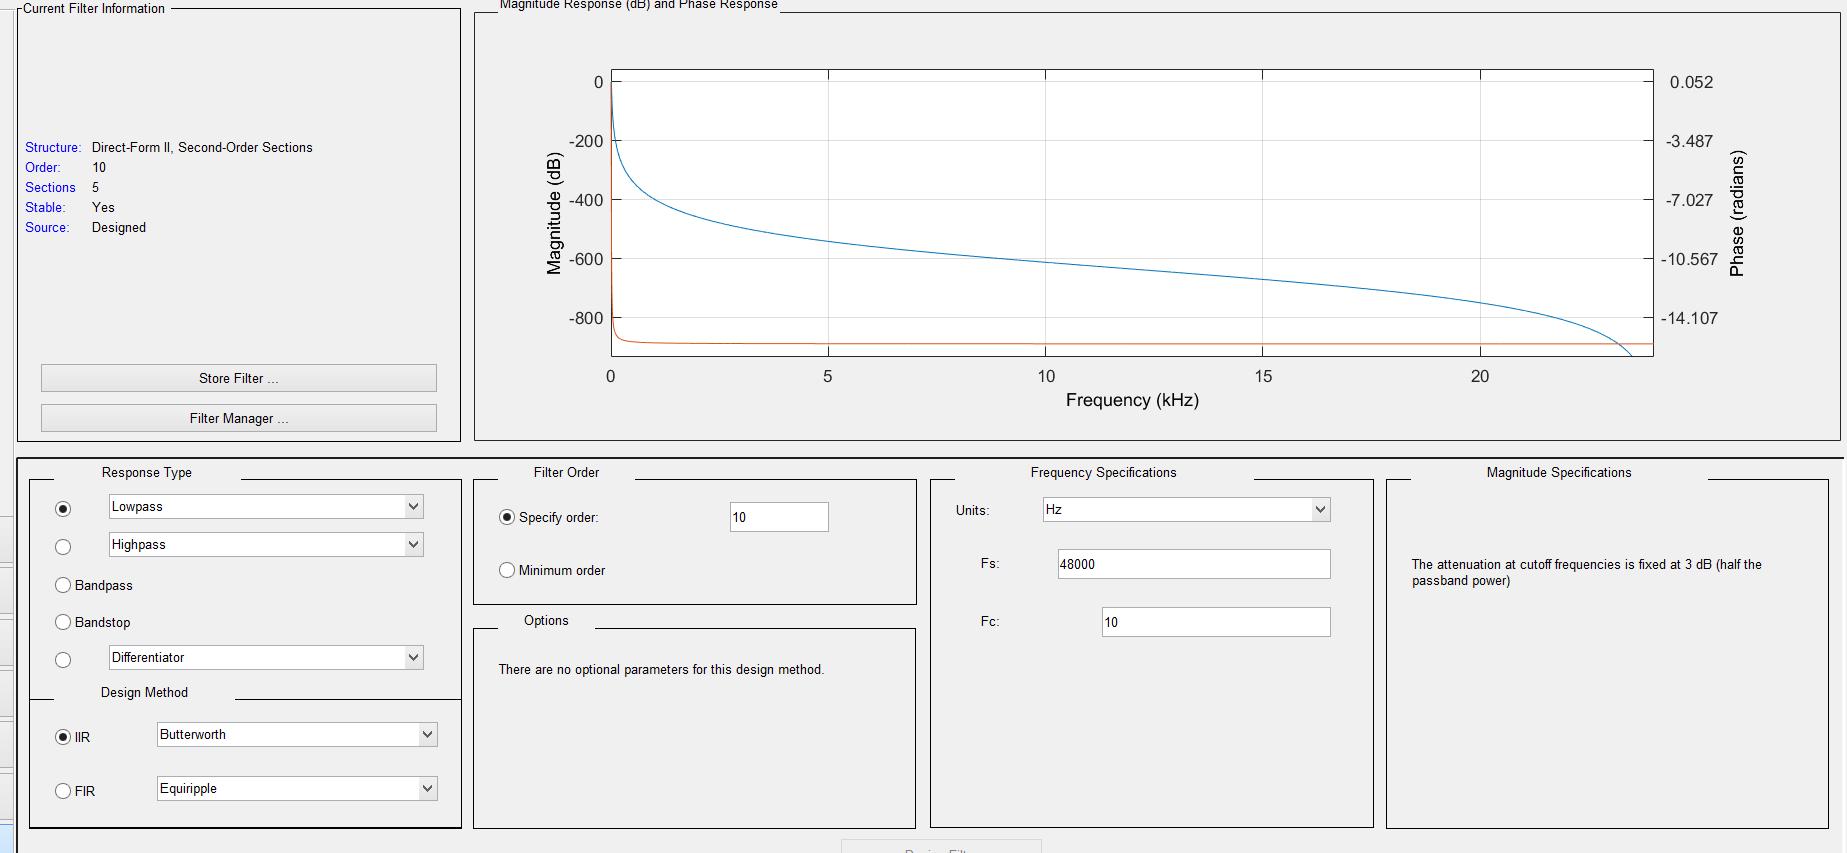
\includegraphics[width=150mm]{figures/FDATool.PNG}
	\caption{Design af IIR lavpas filter i FDA tools i matlab}
	\label{fig:FDAtools}
\end{figure}

Filteret blev desginet med ønske i at skabe et IIR butterworth filter med en knækfrekvens på 10Hz og med en orden på 10. 
Da filteret var designet blev koefficenterne exporteret til et matlab-fil, der blev benyttet i funktionen IIR-lowpass filter.

Koden for IIR lavpas filter funktionen kan ses nedenuner:
    \begin{verbatim}
    function [ output_signal ] = IIR_Lowpass( input_signal )
    %Load koefficenter for designet IIR-filter:
    load LowpassIIR
    
    b=[-1.99958882636935;-1.99881044943430;-1.99814879930370;
    -1.99766835702012;-1.99741586621321];
    a=[0.999590539491295;0.998812161889374;0.998150511191915;
    0.997670068496728;0.997417577473500];
    
    
    output_signal=filter(b,a,input_signal);
    
    
    end
    \end{verbatim}

\subsection{FIR-weight funktion}

Equalizeren blev kørt med forskellige signaler, hvor der blev eksperimenteret med forskellige vægtning af de enkelte Båndpas-filtre samt frekvensbåndet de dækkede. Efter at havde eksperimenteret med de forskellige frekvensbånd blev det bestemt, at de enkelte frekvensbånd skulle dække følgende frekvensområder, der alle ligger i det hørbare frekvensområde:
\begin{itemize}
	\item Bånd 1 -
	\item Bånd 2 -
	\item Bånd 3 -
	\item Bånd 4 -
	\item Bånd 5 -
\end{itemize}

\begin{verbatim}
	
	%Give weights in dB
	function [ output_signal ] = FIR_WEIGHT(input_signal,weight,weight2,weight3,weight4,weight5)
	
	[LP] = IIR_Lowpass(input_signal);
	[BP1, notused] = FIR_bandpass_function(input_signal, 8, 100);
	[BP2, notused] = FIR_bandpass_function(input_signal, 80, 1000);
	[BP3, notused] = FIR_bandpass_function(input_signal, 800, 10000);
	[HP, notused] = FIR_bandpass_function(input_signal, 8000, 20000);
	
	%weight = ln(10)*(x/(20*ln(10)));
	%weight2 = ln(10)*(x/(20*ln(10)));
	%weight3 = ln(10)*(x/(20*ln(10)));
	%weight4 = ln(10)*(x/(20*ln(10)));
	%weight5 = ln(10)*(x/(20*ln(10)));
	
	LP = LP * weight;
	BP1 = BP1 * weight2;
	BP2 = BP2 * weight3;
	BP3 = BP3 * weight4;
	HP = HP * weight5;
	
	output_signal = LP + BP1 + BP2 + BP3 + HP;
\end{verbatim}

\section{Resultat}
I dette afsnit fremstilles resultaterne af at køre Audio Equalizeren på en række forskellige signaler.
